\chapter{Self-Supervised Learning}

\section{Introduction}
Self-Supervised Learning (SSL) is  a particular type of representation learning that enables learning good data representation from \textbf{unlabelled} dataset.

The \textbf{idea} of the SSL is to constructing supervised learning task out of unsupervised dataset.

This make sense for two reason:
\begin{compactitemize}
    \item Data labelling is expensive; thus, the high-quality labeled dataset is limited.
    \item Learning good representation makes transferring useful information to various downstream tasks.
\end{compactitemize}
\begin{figure}[H]
    \centering
    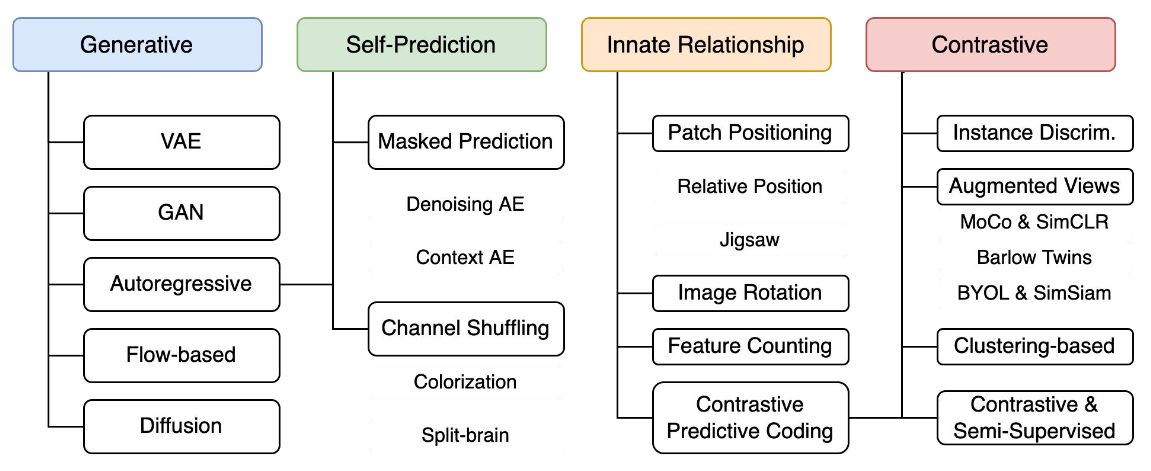
\includegraphics[width=1\textwidth]{images/SS1.png}
    \label{fig:MHA2}
\end{figure}

\subsection{Self-Supervised Learning vs Generative Learning}
Often, we are not really interested to generate pixel-level detail. Instead we are more interested to learn only high-level semantic features through \textbf{pretext task}.
\begin{figure}[H]
    \centering
    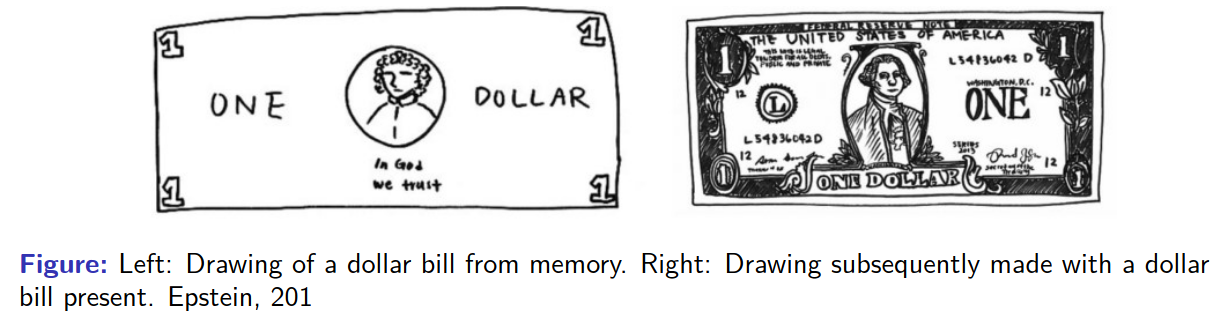
\includegraphics[width=0.85\textwidth]{images/SS2.png}
    \label{fig:MHA2}
\end{figure}

\subsection{Self-Supervised Learning through Pretext Tasks}

Self-supervised learning aims to learn high-level semantic representations from data without relying on manually annotated labels. This is achieved through the use of \textbf{pretext tasks}, which are automatically generated tasks designed to encourage the model to extract meaningful and general features from the data.

One of the main characteristics of a pretext task is that it allows labels to be generated automatically, without any human intervention (e.g., image rotation, colorization, or jigsaw puzzles).

As an example, consider the following \textbf{pretext task}: given an image of a bird, the image is rotated by a certain angle (e.g., $0^\circ$, $90^\circ$, $180^\circ$, $270^\circ$), and the model is trained to \textbf{predict} which rotation has been applied. This results in a simple 4-class classification problem.

In this scenario, the model is a standard \textbf{Convolutional Neural Network (CNN)}. After training the CNN on the pretext task, the network learns to extract useful visual features that capture the structure and semantics of the images. Once training is complete, the feature extractor (i.e., the convolutional layers) can be detached and reused as part of a new model for a downstream task.

Specifically, the pretrained feature extractor is connected to a new Multi-Layer Perceptron (MLP) designed for the target task. Since the CNN has already learned informative representations through the pretext task, only a relatively small amount of labeled data is required to train the new model. This approach partially addresses the problem of limited labeled data by leveraging large amounts of unlabeled data during pretraining.
\begin{figure}[H]
    \centering
    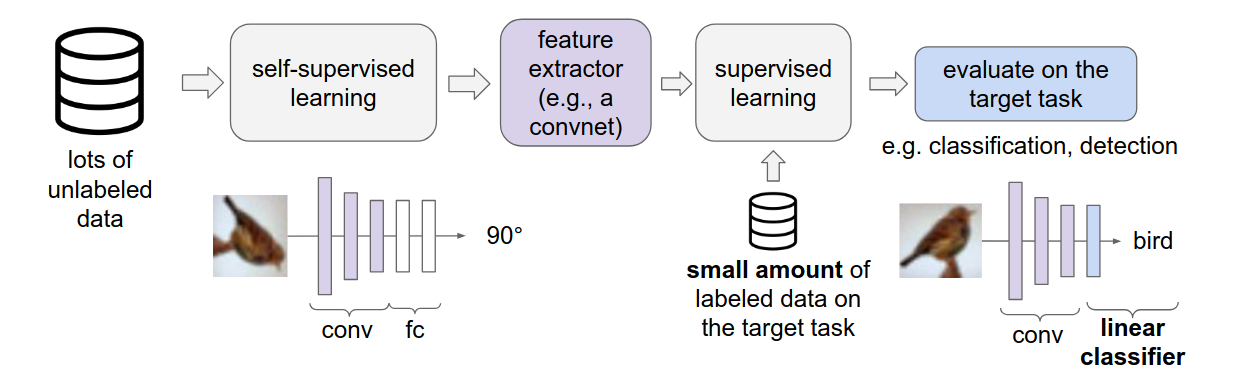
\includegraphics[width=0.9\textwidth]{images/SS3.png}
    \label{fig:MHA2}
\end{figure}
Predicting image rotations is an effective pretext task because it encourages the model to learn meaningful visual representations rather than focusing on low-level cues. In order to correctly infer the rotation applied to an image, the model must develop a form of visual commonsense, that is, an understanding of how objects typically appear in their canonical, unperturbed orientation.

Indeed, recognizing whether an object is upright, upside-down, or rotated by a specific angle requires the network to capture high-level semantic information such as object shape, part configuration, and spatial relationships between components. For example, correctly identifying that an animal is upside-down implies understanding where its head, limbs, and body are normally located. This prevents the model from relying solely on trivial pixel-level statistics and instead pushes it toward learning semantically rich and transferable features.

As a result, rotation prediction acts as a strong supervisory signal without requiring manual annotations. The features learned during this pretraining phase are general and robust, making them well-suited for downstream tasks such as image classification, object detection, or segmentation, even when only a limited amount of labeled data is available.
\begin{wrapfigure}{r}{0.5\textwidth}
    \centering
    \vspace{-10pt}
    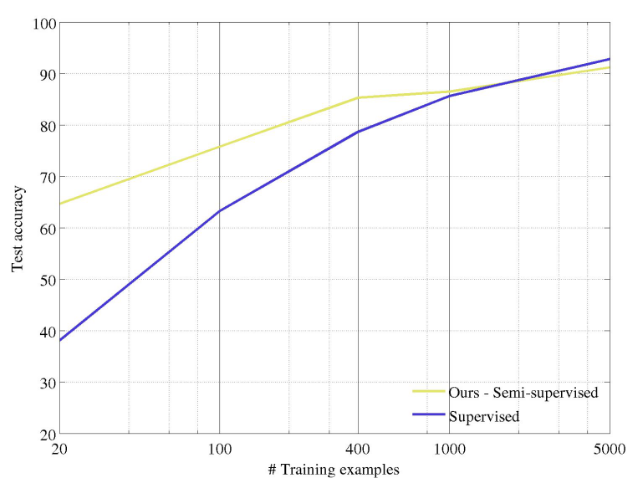
\includegraphics[width=\linewidth]{images/SS4.png}
    \label{fig:Scaled Dot Product Attention}
    \vspace{-10pt}
\end{wrapfigure}
The figure shows that \textbf{self-supervised pretraining} based on rotation prediction enables the model to learn \textbf{robust and transferable visual features}. During the downstream supervised phase, the early layers (\textbf{conv1 and conv2}) are \textbf{frozen}, while only the higher-level layers (\textbf{conv3 and the linear classifier}) are trained using a \textbf{small subset of labeled data}. This setup demonstrates that the representations learned through the pretext task are sufficiently informative to achieve strong performance even with limited supervision.

\section{SLL through intra-example relationships}

\subsection{Pretext Task: Solving ``Jigsaw Puzzles''}

Learning the spatial relationships among image patches is an effective strategy for self-supervised representation learning. In this context, the pretext task consists of dividing an image into a set of patches and training a model to predict their correct relative positions or permutations. Early approaches include predicting the relative position between pairs of patches  and solving jigsaw puzzles constructed from shuffled image patches.
\begin{figure}[H]
    \centering
    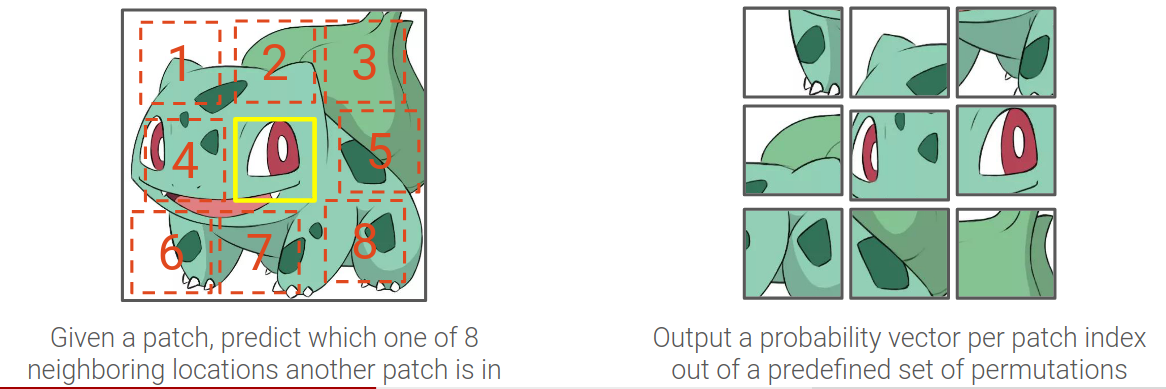
\includegraphics[width=0.9\textwidth]{images/SS5.png}
    \label{fig:MHA2}
\end{figure}
The intuition behind the jigsaw puzzle task is that, to correctly reassemble the image, the model must understand that objects are composed of meaningful parts and learn how these parts are spatially arranged. This encourages the network to capture semantic information about object structure rather than relying on low-level visual cues.

A key challenge of this approach is the inherent ambiguity when considering each patch independently, as multiple configurations may appear locally plausible. To address this issue, the model observes all patches jointly, framing the problem as a global permutation prediction task. Since the placement of each patch is mutually exclusive, jointly reasoning over all tiles significantly reduces ambiguity and leads to the learning of more coherent and informative visual representations .
\begin{figure}[H]
    \centering
    \begin{minipage}{0.35\textwidth}
        \centering
        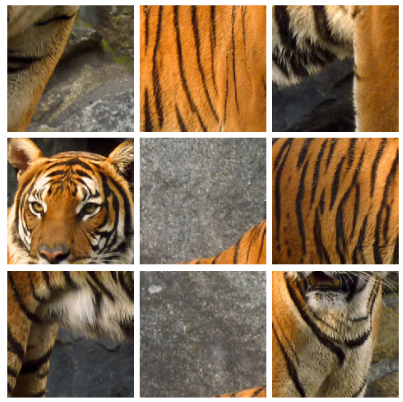
\includegraphics[width=\textwidth]{images/SS6.png}
        \label{fig:Residuals}
    \end{minipage}
    \label{fig:TS_Residuals}
    \hfill
    \begin{minipage}{0.35\textwidth}
        \centering
        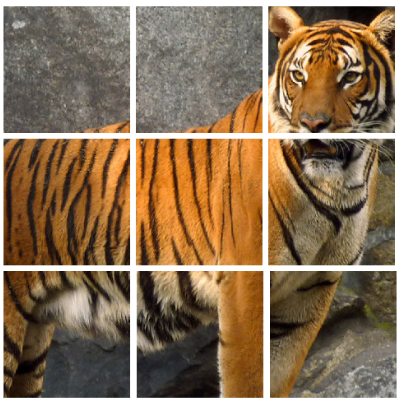
\includegraphics[width=\textwidth]{images/SS7.png}
        \label{fig:Residuals}
    \end{minipage}
    \label{fig:TS_Residuals}
\end{figure}

\subsection{Pretext Task: Predicting Relative Patch Locations}

Predicting the relative spatial arrangement of image patches is an early and influential pretext task for self-supervised representation learning. Given a large collection of unlabeled images, random pairs of patches are extracted from each image and used as input to the model. One patch is treated as a reference, while the second patch is sampled from a neighboring region at a relative position drawn from a predefined set.

The pretext task consists of training a model to predict the relative position of the second patch with respect to the first (e.g., top, bottom, left, right, or diagonal), framing the problem as a classification task. This setup does not require any manual annotations, as the relative spatial relationship between patches is automatically determined during data generation.

The underlying hypothesis is that performing well on this task requires the model to move beyond low-level texture cues and instead learn semantically meaningful representations. In particular, the model is encouraged to recognize objects, their constituent parts, and their typical spatial configurations, since understanding how parts of an object are arranged is crucial for correctly reasoning about relative patch locations.
\begin{figure}[H]
    \centering
    \begin{minipage}{0.5\textwidth}
        \centering
        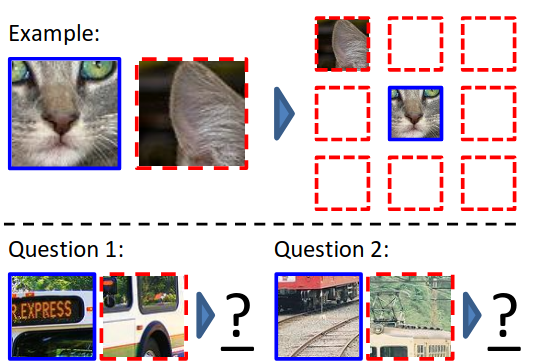
\includegraphics[width=\textwidth]{images/SS8.png}
        \label{fig:Residuals}
    \end{minipage}
    \label{fig:TS_Residuals}
    \hfill
    \begin{minipage}{0.4\textwidth}
        \centering
        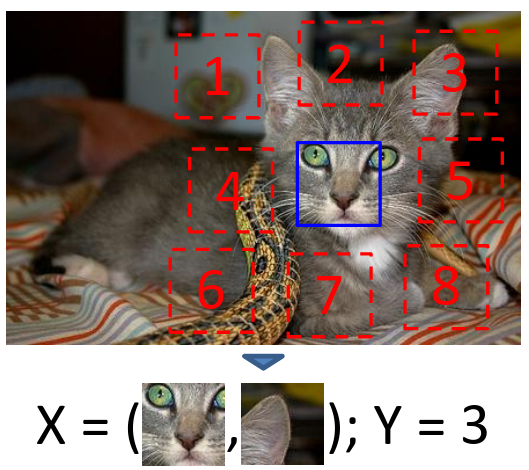
\includegraphics[width=\textwidth]{images/SS9.png}
        \label{fig:Residuals}
    \end{minipage}
    \label{fig:TS_Residuals}
\end{figure}

\subsection{Pretext Tasks: Colorization}
\begin{wrapfigure}{r}{0.2\textwidth}
    \centering
    \vspace{-10pt}
    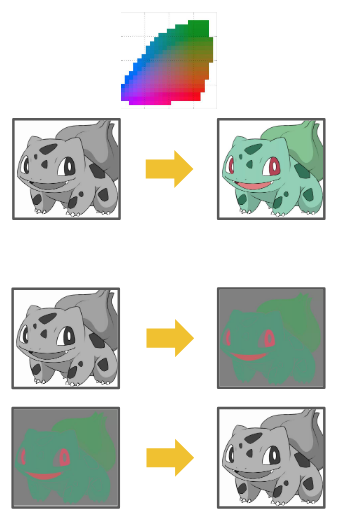
\includegraphics[width=\linewidth]{images/SS10.png}
    \label{fig:Scaled Dot Product Attention}
    \vspace{-10pt}
\end{wrapfigure}
Image colorization is a powerful self-supervised pretext task that consists of predicting color information from grayscale images. In this setting, supervision is obtained directly from the data, since color images can be automatically converted to grayscale. One representative approach is proposed by Zhang et al., where the model is trained to predict the discretized color values in the CIE Lab color space given only the luminance channel. The task is formulated as a classification problem over color bins, which helps the model capture multimodal color distributions.

Colorization encourages the network to learn high-level semantic features, as assigning plausible colors often requires understanding object identity, material properties, and scene context. In particular, correctly colorizing an image implicitly forces the model to distinguish between different object parts (e.g., eyes, skin, hair), to reason about shapes and boundaries, and to separate foreground objects from the background. This process leads the network to capture meaningful structural and spatial information rather than relying solely on low-level texture cues.

A generalization of this idea is the \emph{split-brain autoencoder} introduced by Zhang et al. In this framework, the input channels are divided into two complementary subsets, and the model is trained to predict one subset from the other. For example, the network may predict chrominance from luminance, or more generally, infer color, depth, or other modalities from available visual information. By forcing different subnetworks to learn from partial observations, this approach further promotes the learning of robust and semantically rich representations.

Beyond representation learning, colorization models also have practical applications. Since they are trained using artificially generated grayscale images, they can be directly applied to real legacy black-and-white photographs, producing visually plausible colorized results, as demonstrated in \emph{Colorful Image Colorization} by Zhang et al.
\begin{figure}[H]
    \centering
    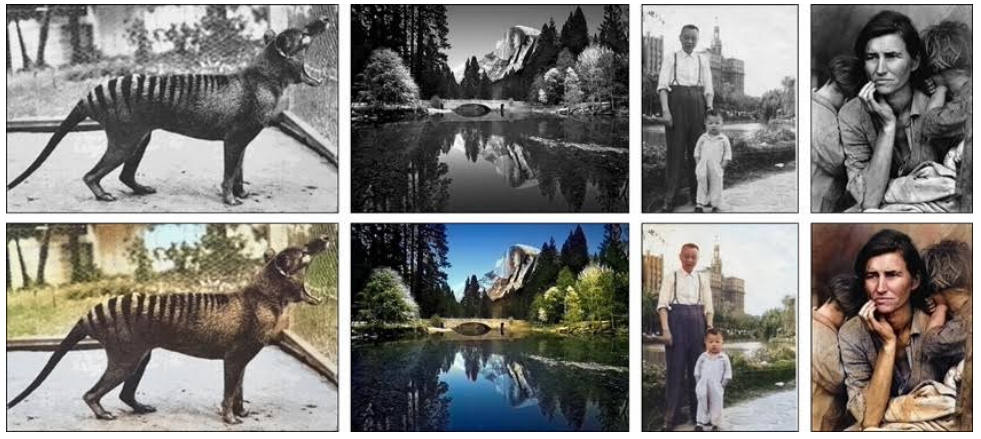
\includegraphics[width=0.7\textwidth]{images/SS11.png}
    \label{fig:MHA2}
\end{figure}

\section{Self-Prediction}
\begin{wrapfigure}{r}{0.25\textwidth}
    \centering
    \vspace{-10pt}
    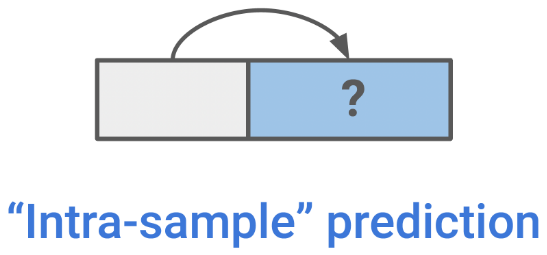
\includegraphics[width=\linewidth]{images/SS12.png}
    \label{fig:Scaled Dot Product Attention}
    \vspace{-10pt}
\end{wrapfigure}
Self-prediction is a branch of \textbf{self-supervised learning} in which, given an individual data sample, the learning task consists of predicting one part of the sample from the remaining parts. The key idea is to artificially define a prediction problem \emph{within} each data sample, without relying on externally provided labels.

\begin{figure}[H]
    \centering
    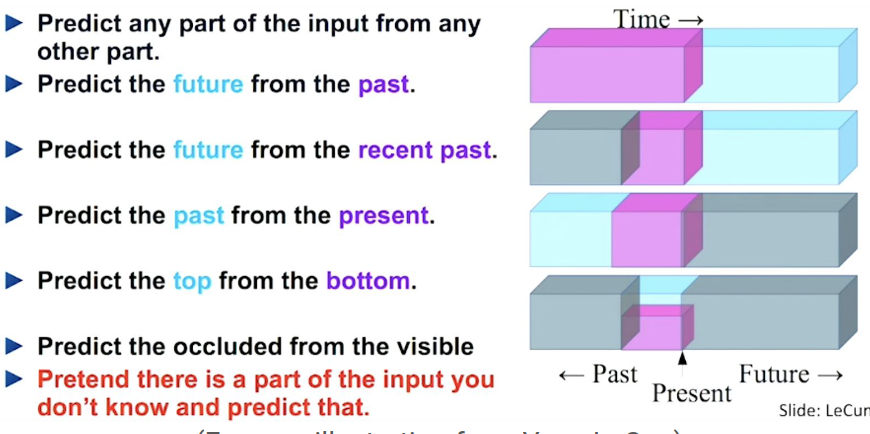
\includegraphics[width=0.6\textwidth]{images/SS13.png}
    \label{fig:MHA2}
\end{figure}
More specifically, a portion of the data is treated as if it were \textbf{missing}, even though it is actually available. The neural network is then trained to predict this missing part using the observed portion of the sample. By doing so, the model is forced to learn meaningful internal representations that capture the structure and dependencies of the data.

In general, self-prediction methods construct prediction tasks directly from the data by pretending that certain parts are unknown and using the remaining parts as input. This principle applies across different data modalities (e.g., images, audio, text) and forms the foundation of several successful self-supervised approaches.

Self-prediction methods can be broadly categorized into three main classes:
\begin{compactitemize}
    \item \textbf{Masked generation}
    \item \textbf{Autoregressive generation}
    \item \textbf{Hybrid self-prediction}
\end{compactitemize}

\subsection{Masked Generation}

Masked generation is a self-prediction strategy in which a random portion of the input data is masked out and treated as missing, independently of any natural ordering in the data. The model is trained to predict the masked portion using the remaining unmasked information, thereby learning dependencies and structure within the data.

This paradigm can be applied across different modalities. In natural language processing, a prominent example is \textbf{masked language modeling}, as used in BERT, where randomly selected tokens are masked and the model is trained to predict them from the surrounding context. In computer vision, masked generation includes tasks such as image inpainting and masked patch prediction, including recent approaches like \textbf{Masked AutoEncoders (MAEs)}.
\begin{figure}[H]
    \centering
    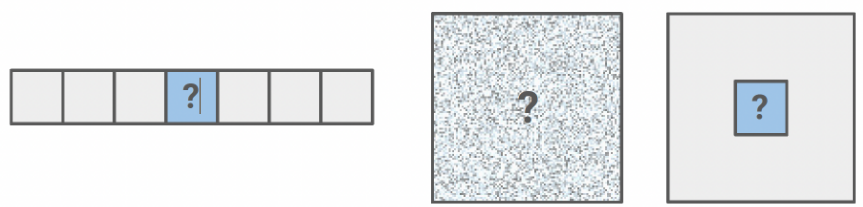
\includegraphics[width=0.6\textwidth]{images/SS14.png}
    \label{fig:MHA2}
\end{figure}
\subsubsection{Self-prediction by Inpainting}

Self-prediction by inpainting consists of predicting the content of an arbitrary missing region in an image based on its surrounding context. In this setting, a portion of the image is removed, and the model is trained to reconstruct the missing pixels using the visible parts of the image \cite{Pathak2016}.

To succeed at this task, the model must capture both local appearance cues and global semantic information. In particular, it needs to understand the overall image content in order to produce a plausible hypothesis for the missing region. As a result, inpainting encourages the learning of representations that encode not only textures and low-level visual features, but also object structure, spatial relationships, and semantic coherence.
\begin{figure}[H]
    \centering
    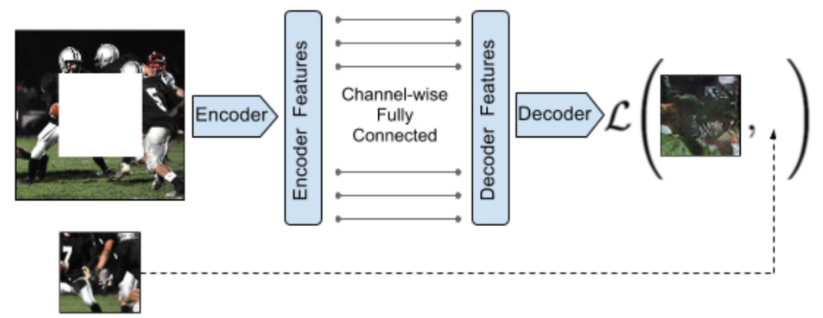
\includegraphics[width=0.7\textwidth]{images/SS15.png}
    \label{fig:MHA2}
\end{figure}
\subsubsection{Self-prediction through Masked AutoEncoders}

Masked AutoEncoders (MAEs) are a self-prediction approach in which random patches of an input image are masked, and the model is trained to reconstruct the missing patches in pixel space. Unlike traditional autoencoders, MAEs adopt an \textbf{asymmetric encoder-decoder architecture}.

The encoder processes only the visible patches and produces a latent representation without using mask tokens, making it computationally efficient. The decoder then takes this latent representation together with mask tokens and reconstructs the full image, including the missing patches. By reconstructing heavily masked inputs, MAEs force the model to learn strong and semantically meaningful visual representations that are well suited for downstream tasks.
\begin{figure}[H]
    \centering
    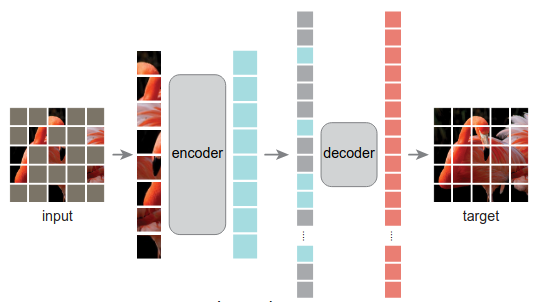
\includegraphics[width=0.6\textwidth]{images/SS16.png}
    \label{fig:MHA2}
\end{figure}
\subsection{Autoregressive Generation}

Autoregressive generation is a self-prediction strategy in which the model predicts future elements of a data sample based on previously observed elements. This approach explicitly exploits the inherent sequential structure of the data and models the joint distribution as a product of conditional probabilities.

Autoregressive models are widely used in domains where data has a natural ordering. Examples include audio generation (e.g., WaveNet, WaveRNN), autoregressive language modeling (e.g., GPT, XLNet), and image modeling by imposing an artificial raster-scan order on pixels or patches (e.g., PixelCNN, PixelRNN, and iGPT).
\begin{figure}[H]
    \centering
    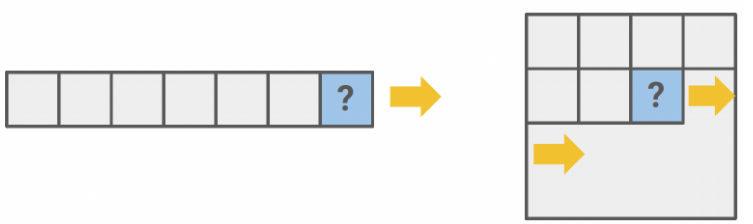
\includegraphics[width=0.6\textwidth]{images/SS17.png}
    \label{fig:MHA2}
\end{figure}

\section{Contrastive Learning}
\section{Contrastive Learning}

Pretext tasks play a central role in self-supervised learning, as they encourage models to acquire meaningful visual representations without relying on human-annotated labels. In particular, they push neural networks to develop a form of \textbf{visual common sense}, enabling the extraction of high-level semantic information that can be effectively reused for downstream tasks. To successfully solve a pretext task, the model is forced to learn informative features of natural images, such as object structure and semantic categories, rather than relying on superficial visual cues. Importantly, the final goal is not to maximize performance on the pretext task itself, but to learn representations that are \textbf{useful and transferable} to downstream applications such as classification, detection, or segmentation.

Despite their effectiveness, pretext-task-based approaches present several limitations. Designing suitable pretext tasks often requires \textbf{significant manual effort} and domain knowledge. Moreover, the learned representations may fail to be sufficiently general, as they can become \textbf{tightly coupled to the specific pretext task} used during training, reducing their applicability across different downstream problems.

These limitations naturally raise the question of whether it is possible to define a more general and task-agnostic self-supervised learning paradigm. \textbf{Contrastive learning} provides a positive answer to this question. Instead of relying on a handcrafted prediction task, contrastive learning learns representations by comparing different views of the data, explicitly encouraging representations of similar samples to be close while pushing apart representations of dissimilar samples. This formulation yields a more flexible and general objective, capable of producing robust and widely transferable visual features.

\begin{figure}[H]
    \centering
    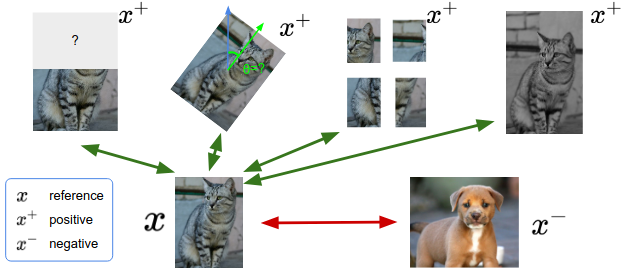
\includegraphics[width=0.8\textwidth]{images/SS18.png}
    \label{fig:MHA2}
\end{figure}

\subsection{Contrastive Representation Learning}

The goal of \textbf{contrastive representation learning} is to learn an embedding space in which semantically similar samples are mapped close to each other, while dissimilar samples are pushed far apart. This objective is achieved by explicitly comparing pairs of samples and enforcing relative similarity constraints in the learned representation space.
\begin{figure}[H]
    \centering
    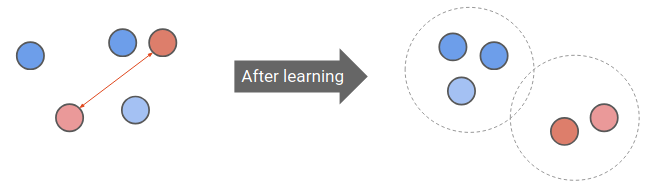
\includegraphics[width=0.6\textwidth]{images/SS20.png}
    \label{fig:MHA2}
\end{figure}
Formally, given an encoder function $f(\cdot;\theta_f)$, a reference sample $x$ (also called an \textbf{anchor}), a \textbf{positive sample} $x^+$ that is semantically related to $x$, and a \textbf{negative sample} $x^-$ that is unrelated, the model is trained such that
\[
\text{score}(f(x), f(x^+)) \gg \text{score}(f(x), f(x^-)).
\]
The score function typically measures similarity in the embedding space, such as cosine similarity or dot product.

Positive samples are usually obtained through \textbf{positive mining strategies}, for example by applying different data augmentations to the same input or by using different views of the same underlying scene or object. Negative samples are drawn from other, unrelated data points within the dataset or the same training batch.

By enforcing these constraints, contrastive learning encourages the encoder to capture high-level semantic features that are invariant to irrelevant transformations, resulting in representations that are robust and highly transferable to downstream tasks.

\subsection{Contrastive Loss}

The contrastive loss was introduced by Chopra et al. as a metric learning objective designed to bring similar samples close in the embedding space while pushing dissimilar samples apart. Unlike self-supervised contrastive learning, this formulation typically assumes the availability of \textbf{labeled data}, where samples from the same class are considered similar and samples from different classes are considered dissimilar.

Given an encoder function $f(\cdot;\theta_f)$ and a pair of labeled samples $(x_i, x_j)$, the contrastive loss is defined as:
\[
\mathcal{L}(x_i, x_j; \theta_f) =
\begin{cases}
\| f(x_i) - f(x_j) \|, & \text{if } i = j ,(minimize) \\
\max\left(0, \alpha - \| f(x_i) - f(x_j) \| \right), & \text{if } i \neq j ,(maximize)
\end{cases}
\]
where $\alpha$ is a positive margin that controls the minimum desired distance between embeddings of samples belonging to different classes.

For positive pairs (i.e., samples from the same class), the loss encourages minimizing the distance between their embeddings. For negative pairs, the loss penalizes embeddings that are closer than the margin $\alpha$. If the distance between two negative samples exceeds the margin, their contribution to the loss is zero.

The introduction of the margin is crucial to prevent \textbf{representation collapse}, a degenerate solution in which all samples are mapped to the same point in the embedding space. By enforcing a minimum separation between negative pairs, contrastive loss promotes a structured and discriminative embedding space.

\subsection{Triplet Loss}

The triplet loss is a metric learning objective that extends the contrastive loss by jointly considering three samples at a time: an \textbf{anchor} sample $x$, a \textbf{positive} sample $x^+$ belonging to the same class as the anchor, and a \textbf{negative} sample $x^-$ belonging to a different class. The objective is to learn an embedding space in which the anchor is closer to the positive sample than to the negative one.

More formally, the desired constraint is that the distance between the anchor and the positive sample is smaller than the distance between the anchor and the negative sample by at least a margin $\alpha$:
\[
\| f(x) - f(x^+) \|_2^2 + \alpha < \| f(x) - f(x^-) \|_2^2.
\]

This constraint is enforced by minimizing the following loss function:
\[
\mathcal{L}(x, x^+, x^-; \theta_f) =
\max\left(0,
\| f(x) - f(x^+) \|_2^2
-
\| f(x) - f(x^-) \|_2^2
+ \alpha
\right).
\]

If the constraint is satisfied, the loss is zero; otherwise, the model is penalized proportionally to how much the margin is violated. By jointly optimizing distances between anchor--positive and anchor--negative pairs, the triplet loss encourages a well-structured and discriminative embedding space.

\begin{figure}[H]
    \centering
    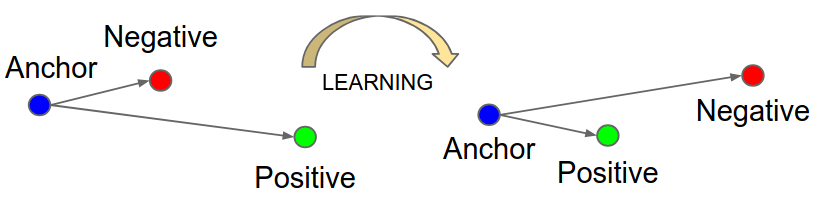
\includegraphics[width=0.6\textwidth]{images/SS21.png}
    \label{fig:MHA2}
\end{figure}

\subsection{InfoNCE}

The InfoNCE loss is a widely used objective in contrastive representation learning that formulates the learning problem as a \textbf{classification task}. Given an anchor sample $x$ and its corresponding positive sample $x^+$, the model is trained to identify the positive sample among a set of other unrelated samples, which act as \textbf{negative examples}.

More concretely, for each anchor $x$, one positive pair $(x, x^+)$ and $N-1$ negative samples $\{x^-_j\}_{j=1}^{N-1}$ are considered. Using an encoder function $f(\cdot; \theta_f)$ and a similarity function $\text{sim}(\cdot, \cdot)$, the InfoNCE loss is defined as:
\[
\mathcal{L}_{\text{InfoNCE}}(x; \theta_f) =
- \log
\frac{
\overbrace{\exp\left(\text{sim}(f(x), f(x^+))\right)}^{\text{score for the positive pair}}
}{
\underbrace{
\exp\left(\text{sim}(f(x), f(x^+))\right)
}_{\text{score for the positive pair}}
+
\underbrace{
\sum_{j=1}^{N-1}
\exp\left(\text{sim}(f(x), f(x^-_j))\right)
}_{\text{score for the $N-1$ negative pairs}}
}
\]

Intuitively, the model is encouraged to assign a higher similarity score to the positive pair than to all negative pairs. This formulation is equivalent to the standard \textbf{categorical cross-entropy loss} applied to an $N$-way softmax classifier, where the goal is to correctly identify the positive sample among a finite set of candidate samples.

Thanks to this formulation, InfoNCE scales naturally with the number of negative samples and has become the de facto standard loss in modern self-supervised contrastive learning methods.

\subsection{SimCLR: a simple framework}
\begin{figure}[H]
    \centering
    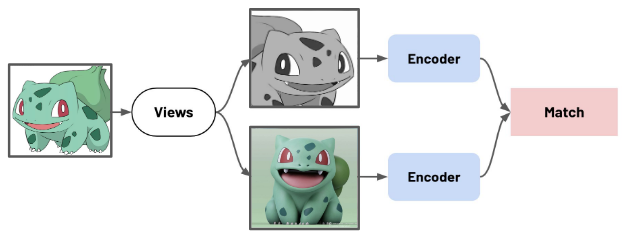
\includegraphics[width=0.6\textwidth]{images/SS22.png}
    \caption{SimCLR}
    \label{fig:MHA2}
\end{figure}

\begin{wrapfigure}{r}{0.35\textwidth}
    \centering
    \vspace{-10pt}
    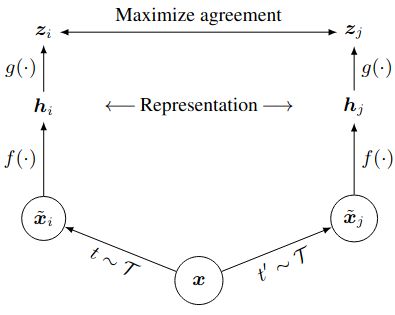
\includegraphics[width=\linewidth]{images/SS23.png}
    \label{fig:Scaled Dot Product Attention}
    \vspace{-10pt}
\end{wrapfigure}
SimCLR (Simple Framework for Contrastive Learning of Visual Representations) is a self-supervised contrastive learning framework that learns visual representations by maximizing agreement between different augmented views of the same data sample.

Given an input image $x$, two stochastic data augmentation operators $t \sim \mathcal{T}$ and $t' \sim \mathcal{T}$ are independently sampled from a family of transformations and applied to obtain two correlated views:
\[
\tilde{x}_i = t(x), \quad \tilde{x}_j = t'(x).
\]
These two views form a \textbf{positive pair}, while views obtained from different images naturally act as \textbf{negative samples}.

Each augmented image is processed by a shared \textbf{encoder network} $f(\cdot)$, producing intermediate representations:
\[
h_i = f(\tilde{x}_i), \quad h_j = f(\tilde{x}_j).
\]
The representations are then mapped by a \textbf{projection head} $g(\cdot)$, typically implemented as a multilayer perceptron, yielding the embeddings used for contrastive learning:
\[
z_i = g(h_i), \quad z_j = g(h_j).
\]

A key aspect of SimCLR is that it does \textbf{not explicitly sample negative examples}. Given a mini-batch of $N$ images, two augmented views are generated for each image, resulting in a total of $2N$ samples. For a given anchor representation, the corresponding positive sample is the other augmented view of the same image, while the remaining $2(N-1)$ augmented views in the batch act as negative samples. This explains the appearance of $2N$ terms in the contrastive loss formulation.

The similarity between two embeddings is measured using the \textbf{cosine similarity}, defined as:
\[
\text{sim}(u, v) = \frac{u^\top v}{\|u\| \, \|v\|},
\]
which focuses on the angular distance between normalized embeddings and has been shown to stabilize and improve contrastive training. 

The contrastive objective is formulated using the \textbf{InfoNCE loss} with a temperature parameter $\tau$. Given a positive pair $(i,j)$ within a batch of $2N$ augmented samples, the loss for sample $i$ is:
\[
\ell_{i,j} =
- \log
\frac{
\exp\left(\text{sim}(z_i, z_j) / \tau\right)
}{
\sum_{k=1}^{2N} \mathbb{1}_{[k \neq i]}
\exp\left(\text{sim}(z_i, z_k) / \tau\right)
},
\]
where $\mathbb{1}_{[k \neq i]}$ excludes the anchor itself from the denominator.

The final SimCLR objective is obtained by symmetrizing the loss over all positive pairs in the batch:
\[
\mathcal{L}_{\text{SimCLR}} =
\frac{1}{2N}
\sum_{i=1}^{N}
\left(
\ell_{i,j(i)} + \ell_{j(i),i}
\right).
\]

An important design choice in SimCLR is the use of the projection head $g(\cdot)$. By applying the contrastive loss in the projection space rather than directly on the encoder output $h$, the encoder $f(\cdot)$ is encouraged to preserve more general and transferable information. After pretraining, the projection head is discarded, and only the encoder $f(\cdot)$ is retained for downstream tasks.

\subsubsection{Linear Evaluation on SimCLR Features}
\begin{wrapfigure}{r}{0.45\textwidth}
    \centering
    \vspace{-10pt}
    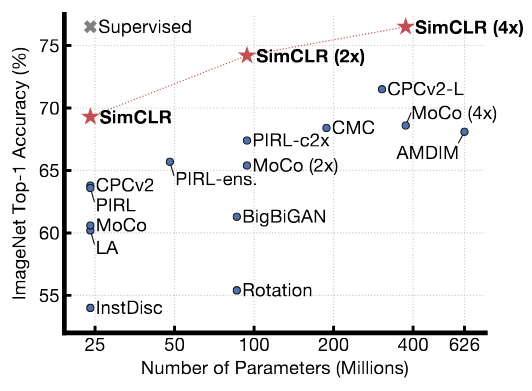
\includegraphics[width=\linewidth]{images/SS24.png}
    \label{fig:Scaled Dot Product Attention}
    \vspace{-10pt}
\end{wrapfigure}
This figure reports the performance of SimCLR representations evaluated through the \textbf{linear evaluation protocol}. The feature encoder is first pretrained on the entire ImageNet dataset using SimCLR, after which it is \textbf{frozen} and a linear classifier is trained on top using labeled data. The results show that SimCLR achieves performance comparable to, and in some cases surpassing, supervised pretraining, highlighting the quality and transferability of the learned representations.

\subsubsection{Linear Evaluation on SimCLR Features}
\begin{wrapfigure}{r}{0.45\textwidth}
    \centering
    \vspace{-10pt}
    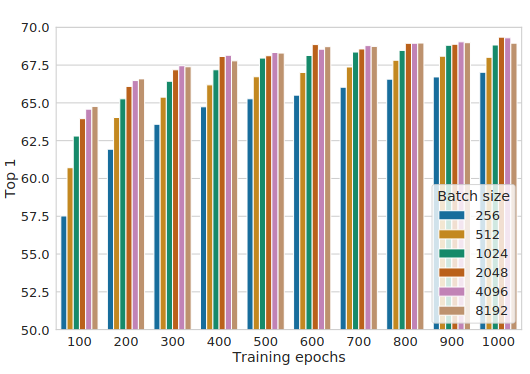
\includegraphics[width=\linewidth]{images/SS25.png}
    \label{fig:Scaled Dot Product Attention}
    \vspace{-10pt}
\end{wrapfigure}
This figure reports the performance of SimCLR representations evaluated through the \textbf{linear evaluation protocol}. The feature encoder is first pretrained on the entire ImageNet dataset using SimCLR, after which it is \textbf{frozen} and a linear classifier is trained on top using labeled data. The results show that SimCLR achieves performance comparable to, and in some cases surpassing, supervised pretraining, highlighting the quality and transferability of the learned representations.
